\subsection*{Studying the Effects of Self-Attention for Medical Image Analysis}

% \subsection*{Ссылка} \url{https://arxiv.org/abs/2109.01486}
\subsubsection*{Введение}
Одна из главных когнитивных способностей, которой обладает хорошо обученный 
специалист в своей предметной области - это внимание или способность \glqq фокусироваться \grqq .
Внимание - это когда человеческий мозг во время обработки информации также 
оценивает релевантность входных признаков. Данный когнитивный процесс 
позволяет концентрироваться на отдельно выбранном признаке и не учитывать другие.
В медицине, к примеру при интерпретации рентгеновских изображений легких
специалист зачастую фокусируется подсознательно, автоматически оценивая 
клинически важные визуальные признаки, используя знания о симптомах пациента и показаниях
к исследованию. Способность искусственно воспроизвести человеческие 
когнитивные способности с помощью нейронных сетей позволит увеличить точность и 
устойчивость предсказаний. В данной работе \cite{ann16} оценивается важность применения self-attention механизмов 
совместно со стандартными моделями компьютерного зрения в медицине.
\subsubsection*{Основная идея}
Стандартные и широко используемые сверточные нейронные сети (СНС) в разрезе 
когнитивных способностей, выделяют наиболее общие признаки и не дают гарантии в 
извлечении релевантной клинической информации. Self-attention мезанизмы, которые способны 
фокусироваться на важных признаках, обучаются от начала и до конца на вместе 
с backbone архитектурой СНС, не внося изменений в процесс обучения. Авторы представляют 
экспериментальную настройку сети, в которой используется стандартная сеть ResNet-18, для 
проведения множества экспериментов на разных медицинских датасетах (данных различной модальности),
в которой увеличиваются residual блоки для размещения трех state-of-the-art 
механизмов внимания (CBAM, SE, GC). Валидация проводилась с использованием стандартной метрики AUC-ROC 
и по качественным визуализациям тепловых карт. \\
\begin{minipage}{1.0\linewidth}
    \begin{center}
        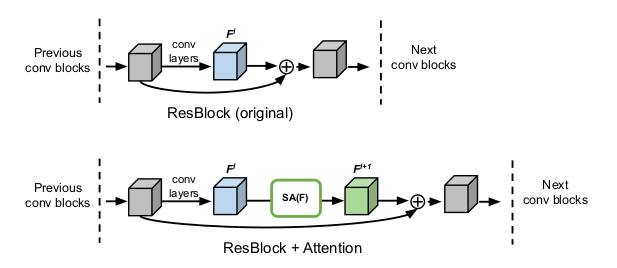
\includegraphics[scale=0.6]{ann16_arch.png} \\
        % \caption{\scriptsize{
        %     Размещение attention механизмов в residual блоках.
        % }}
    \end{center}
    
\end{minipage}
\subsubsection*{Данные}
Skin Dataset, CXR Dataset, MRI Dataset, CT Dataset
\subsection*{Результаты}

\begin{minipage}{0.49\linewidth}
    \begin{center}
        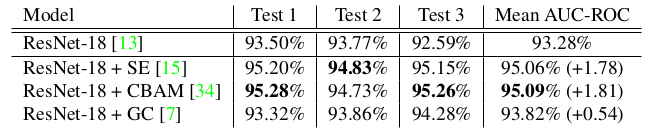
\includegraphics[scale=0.35]{ann16_res1.png} \\
        % \caption{\scriptsize{
        %     Количественные результаты на датасете рака кожи.
        % }}
    \end{center}
    
\end{minipage}
\begin{minipage}{0.49\linewidth}
    \begin{center}
        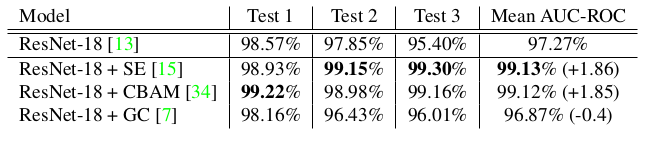
\includegraphics[scale=0.35]{ann16_res2.png} \\
        % \caption{\scriptsize{ 
        %     Количественные результаты на снимках легких.}}
    \end{center}
    
\end{minipage} 


\begin{minipage}{0.49\linewidth}
    \begin{center}
        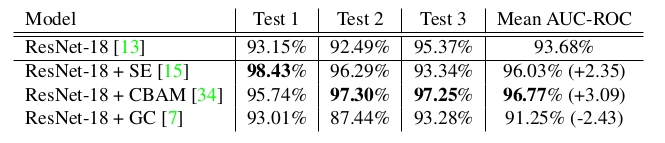
\includegraphics[scale=0.35]{ann16_res3.png} \\
        % \caption{\scriptsize{
        %     Количественные результаты на МРТ-датасете.
        % }}
    \end{center}
    
\end{minipage}
\begin{minipage}{0.49\linewidth}
    \begin{center}
        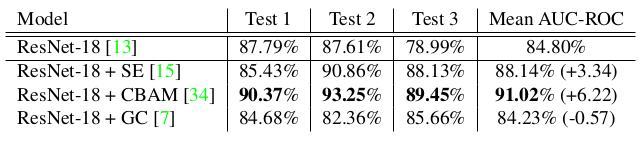
\includegraphics[scale=0.35]{ann16_res4.png} \\
    %     \caption{\scriptsize{ 
    %         Количественные результаты на КТ-датасете.}}
    \end{center}
    
\end{minipage} 


\begin{minipage}{1.0\linewidth}
    \begin{center}
        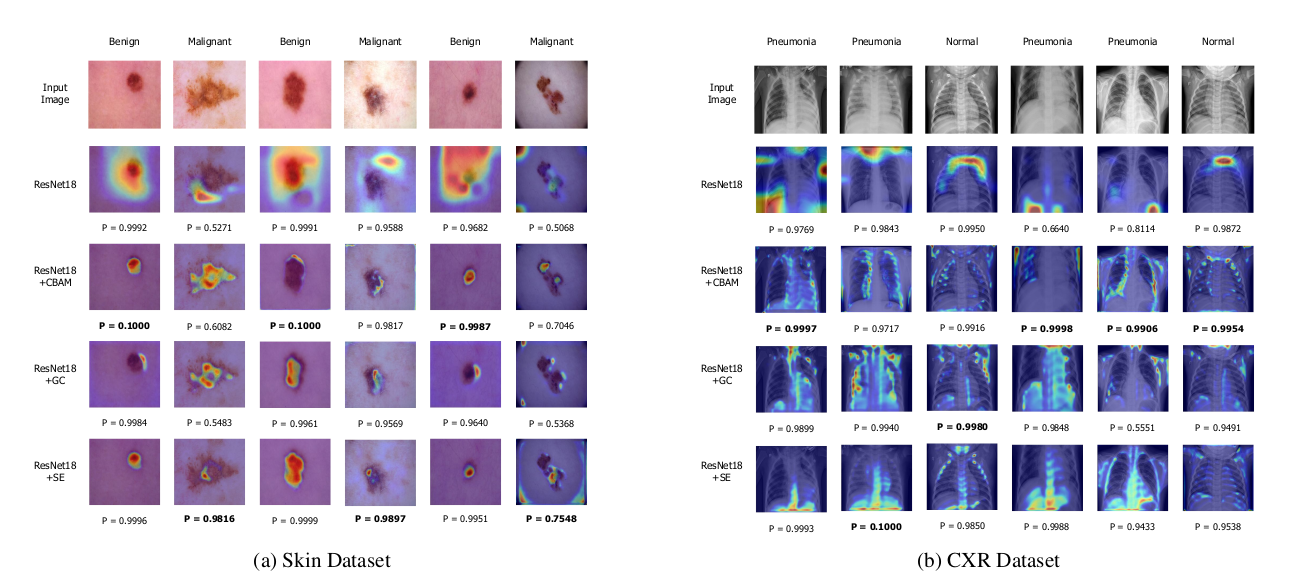
\includegraphics[scale=0.3]{ann16_heatmap.png} \\
        % \caption{\scriptsize{
        %     Визуализация тепловых карт применения каждой модели на данных из датасетов 
        %     рака кожи и рентгеновских снимков.
        % }}
    \end{center}
    
\end{minipage} 
\subsubsection*{Заключение}
В данной статье оценивались различные self-attention механизмы в 
системах медицинского компьютерного зрения. Механизм внимания позволяет 
стандартным СНС больше фокусироваться на семантически важном и релевантном 
содержимом признаков. Использование self-attention механизма улучшило AUC-ROC  
точность предсказания на снимках из всех использованных датасетов. 
